\documentclass[12pt,a4paper]{article}
\usepackage[utf8]{inputenc}
\usepackage{amsmath}
\usepackage{amsfonts}
\usepackage{amssymb}
\usepackage{tikz}
\usepackage{graphicx}
\usetikzlibrary{positioning}
\usepackage{tabularx}

\usepackage{hyperref}
\usepackage{color}
\hypersetup{
	colorlinks,
	filecolor=black,
	linkcolor=black,
	urlcolor=black
}

\usepackage{listings}
%\usepackage[table]{xcolor}
%\setlength{\parindent}{0cm}

%TODO : Eclipse debugging
%     : Ableitungsbaum Beispiel verschönern
%     : 

\begin{document}
\tableofcontents

\newpage
%\newpage
\section{EBNF}
\subsection{Definitionen}
\begin{tabularx}{\linewidth}{r X}
\textbf{EBNF Regel} & \\
\textbf{EBNF Beschreibung} & Eine Menge von EBNF Regeln. Reihenfolge unwichtig.\\
\textbf{LHS/RHS} & Left-hand side, right-hand side\\
\textbf{Control Forms} & Eine der folgenden Begriffe:\\
& Aufreihung, Auswahl, Option, Wiederholung\\
\quad \quad \textbf{Aufreihung} & \textit{room} $\Leftarrow$ D28\\
& \textit{room} $\Leftarrow$ \textit{floor} \textit{number}\\
\quad \quad \textbf{Auswahl} & \textit{bit} $\Leftarrow 0 \mid 1$\\
\quad \quad \textbf{Option} & \textit{initials} $\Leftarrow$ T[R]G\\
\quad \quad \textbf{Wiederholung} & \textit{number} $\Leftarrow$ \{\textit{digit}\}\\
\textbf{Äquivalenz} & Beschreibungen, die dieselben legalen und illegalen Symbole erkennen, sind äquivalent.\\
\textbf{Syntax} & Form. EBNF beschreibt nur die Syntax.\\
\textbf{Semantik} & Bedeutung\\ %TODO mention Legalität in synt or sem
\textbf{Rekursion} & LHS erscheint in der RHS\\
\textbf{Indirekte Rekursion} & Eine folge von Regeln $R_1, \hdots, R_k$ so dass sie einen Rekursiven 'Zyklus' bilden ($R_i$ ruft $R_{i+1}$ auf, und $R_k$ ruft $R_1$ auf).
\end{tabularx}
\newpage
\subsection{Legalität}
\subsubsection{Formeller Beweis: Tabelle}
Jede Zeile wird aus der Vörgängerzeile durch eine der folgenden Regeln abgeleitet:\\
\begin{tabularx}{\linewidth}{l X}
1. & Ersetze einen Namen (LHS) durch die entsprechende Definition (RHS)\\
2. & Wahl einer Alternative\\
3. & Entscheidung ob ein optionales Element dabei ist oder nicht\\
4. & Bestimmung der Zahl der Wiederholungen
\end{tabularx}\\\\
Manchmal werden 1. und 2. gleichzeitig ausgeführt.
\subsubsection{Beispiel: Tabelle}
+128 ist ein integer\\\\
\begin{tabularx}{\linewidth}{l X}
\textit{integer} & \\
$[+\mid-]$ \textit{digit} \{\textit{digit}\} & LHS durch RHS, \textit{integer} wurde ersetzt.\\
+ \textit{digit} \{\textit{digit}\} & Auswahl "+"\\
+ 1 \{\textit{digit}\} & LHS durch RHS, \textit{digit} wurde ersetzt.\\
+ 1 \textit{digit} \textit{digit} & Zweifache Wiederholung ausgewählt.\\
+ 1 2 8 & LHS durch RHS, zwei \textit{digit}s wurden ersetzt.
\end{tabularx}
\subsubsection{Formeller Beweis: Ableitungsbaum}
Graphische Darstellung einer Tabelle. Jeder Zwischenschritt wird als 'Level' des Baums dargestellt. Die Kanten zeigen welche Regeln uns erlauben, von einem Level zum nächstem zu gelangen.
\subsubsection{Beispiel: Ableitungsbaum} %TODO this looks horrible
\begin{figure}[h!]
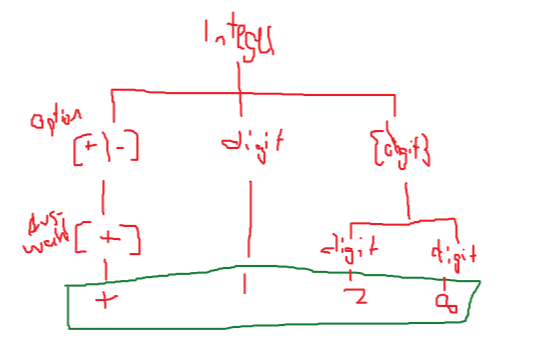
\includegraphics[width=200px]{ableitungsbaum-bsp.png}
\end{figure}
\subsection{Rekursion}
\textit{sequence} $\Leftarrow$ B $\mid$ A\textit{sequence} ergibt "B", "AB", "AAB", $\hdots$\\\\
\textbf{Jede Wiederholung ist eine Rekursion} / kann als Rekursion ausgedrückt werden.\\
\textbf{Nicht jede Rekursion ist eine Wiederholung} / kann man nicht zwingend als Wiederholung ausdrücken.
\subsection{Äquivalenz/Gleichwertigkeit}
Zwei EBNF Beschreibungen sind äquivalent falls sie dieselben legalen und illegalen Symbole erkennen.\\
\begin{tabularx}{\linewidth}{l X}
$\iff$ & Jedes mögliche Symbol, dass eine Regel beschreibt, wird von der anderen als legal bezeichnet, und jedes Symbol dass als illegal erkannt wird wird auch von der anderen als solches erkannt.\\
& Und vice versa. %TODO
\end{tabularx}
\subsection{Sonderzeichen}
Die folgenden 8 Zeichen haben besondere Bedeutungen in EBNF Beschreibungen:\\
\hspace*{1cm} \{, \}, [, ], $\mid$, (, ), $\Leftarrow$\\
Um diese Zeichen in einer Beschreibung zu benutzen, umrahmt man sie.\\
\hspace*{1cm} \fbox{\{}, \fbox{$\mid$}, $\hdots$\\
Man kann auch das Zeichen mit "" umschreiben. In diesem Fall ist auch " ein Sonderzeichen.\\ %TODO
\hspace*{1cm} "\{", "$\mid$", $\hdots$
\newpage
\section{Boolsche Auswertung}
Java wertet zuerst der linke aus, und via "Kurzschluss" schliesst die Entscheidung so bald wie möglich ab.\\
\hspace*{1cm} Z.B. für "\&\&" sobald ein Teil (term) falsch ist.\\
\hspace*{1cm} Für "$\|$" sobald ein Teil (term) wahr ist.\\\\
Implikationen:\\
\begin{tabularx}{\linewidth}{l X}
if((a/b $>$ 0) \&\& (b != 0)) \{\} & Möglicher ArithmeticException weil $a/b$ zuerst ausgewertet wird.\\
if((b != 0) \&\& ($a/b > 0$)) \{\} & Falls b=0, wird der rechte Teil nie ausgewertet, also kann der Rest des codes problemlos weiter ausgeführt werden.\\
if((a $<$ b $\|$ a++ $<$ 5)) \{\} & Falls a$<$b, wird a++ nicht durchgeführt, und dadurch wird im rest des codes a eins weniger sein als erwartet.
\end{tabularx}
\newpage
\section{Packages}
package packageName;\\
import packageName.*;\\\\
Klasse mit Namen D in Package a.b.c sollte in a/b/c/D.class gespeichert sein (relativ zu Root von Projekt)
\subsection{Beispiele}
\begin{lstlisting}[language=Java]
	package pacman.model;
	public class Ghost extends Sprite { }

	//Files Ghost.java und Sprite.java
	//sollten im Folder pacman/model sein


	package pacman.gui;
	import pacman.model.*;

	public class PacManGui {
		Ghost blinky = new Ghost();
	}
\end{lstlisting}
\newpage
\section{Access Modifiers}
\begin{tabularx}{\linewidth}{ l X }
\textbf{public} & Sichtbar für alle anderen Klassen.\\
\textbf{private} & Sichtbar nur in dieser Klasse (und ggf. in eingeschlossenen Klassen/Typen).\\
\textbf{protected} & Sichtbar nur in dieser Klasse, allen Unterklassen der Klasse, und allen anderen Klassen/Typen die in dieser Package deklariert sind.\\
\textbf{default} (package) & Sichtbar in dieser Klasse und allen anderen Klassen/Typen die in dieser Package deklariert sind.
\end{tabularx}
\section{Hoare Tripel}
\subsection{Basics} %TODO translate this
\subsubsection{Allgemeine Form}
$\{P\} S \{Q\}$
\subsubsection{Terminologie}
\begin{tabularx}{\linewidth}{r X}
\textbf{Precondition} & Die Annahme/Aussage, die vor der Ausführung eines Statements (bez. Programmsegments) gilt.\\
\textbf{Postcondition} & Die Aussage, die nach der Ausführung gilt, unter der Annahme dass die Aussage davor gültig ist.
\end{tabularx}
\subsubsection{Forwärts Schliessen}
Von dem Zustand \textbf{vor} der Ausführung eines Programm(segment)s, nimmt man die \textbf{precondition P} an.\\\\
Forwärts Schliessen:
\begin{itemize}
\item Bestimmt was sich aus den ursprünglichen Annahmen herleiten lässt.
\item Ist sehr praktisch wenn eine \textbf{Invariante} gelten soll. (Siehe 5.3) %TODO how to link dynamically? Should be while-loops.
\item Simuliert die Ausführung des Programms für viele "Inputs" "gleichzeitig".
\end{itemize}
\newpage
\subsubsection{Rückwärts Schliessen}
Man wählt einen beliebigen Zustand \textbf{nach} der Ausführung eines Programm(segment)s. Dies ist die \textbf{Postcondition Q}.\\\\
Rückwärts Schliessen:
\begin{itemize}
\item Bestimmt hinreichende Bedingungen die ein Ergebnis garantieren.
\item Wenn das Ergebnis erwünscht ist, dann folgt aus den Bedingungen die Korrektheit.
\item Ist das Ergebnis unerwünscht, dann reichen die Bedingungen um einen Bug zu generieren.
\item Ist oft von grossem praktischem Nutzen. Man muss verstehen, was jede Anweisung zum Erreichen eines bestimmten Zustandes beiträgt.
\end{itemize}
\subsection{If-Statements}
\subsubsection{Allgemeine Form}
\begin{tabularx}{\linewidth}{r X}
\textbf{Form} & $\{P\}$ if $\{b\}$ $S1$ else $S2$ $\{Q\}$\\
\textbf{Precondition} & Das Ergebnis des Tests $b$.\\
\textbf{Postcondition} & Die Disjunktion ("oder") der Postconditions des then- und else-Blockes.
\end{tabularx}
\subsubsection{Gültigkeit}
Gültig genau dann, wenn es $\{Q_1, Q_2\}$ gibt, so dass folgendes gilt:\\\\
\begin{tabular}{ll}
$\{P \land b\}$ $S1$ $\{Q_1\}$\\
$\{P \land \neg b \}$ $S2$ $\{Q_2\}$\\
$Q_1 \lor Q_2 \implies Q$
\end{tabular}
\subsubsection{Übliche Notation}

\subsection{While-Loops}
\subsubsection{Allgemeine Form}
\begin{tabularx}{\linewidth}{r X}
\textbf{Form} & $\{P\}$ while $(b)$ $S$; $\{Q\}$\\ %TODO B or b?
\textbf{Precondition} & \\
\textbf{Postcondition} & \\
\textbf{Invariante} & Eine Aussage, die vor und nach der ausführung jeder Iteration gilt.
\end{tabularx}
\subsubsection{Gültigkeit}
Gültig genau dann, wenn es eine \textbf{Invariante I} gibt, so dass:\\\\
\begin{tabularx}{\linewidth}{lX}
$P \implies I$ & Invariante gilt zu beginn.\\
$\{I \land B\} S \{I\}$ & Nach ausführen des Rumpfes gilt die Invariante wieder.\\
$\{I \land \neg B\} \implies Q$ & Invariante (und Verlassen der Schleife, d.h. test B ist false) impliziert postcondition $Q$.
\end{tabularx}
\section{Extras}
\subsection{Terneary}
Form:\\
\begin{verbatim}
i = input > MAX ? MAX : input;
\end{verbatim}
ergibt (i=max) falls input$>$MAX, sonst (i=input).
\subsection{String Operands}
\begin{tabularx}{\linewidth}{l X}
.toUpperCase / .toLowerCase\\
.indexOf("a") & int Position im String\\
.subString(a, b) & String mit Buchstaben von (int) a zu b (inkl.)\\
.equals(String)\\
.equalsIgnoreCase(String)\\
.startsWith(String) / .endsWith(String)
\end{tabularx}
\subsection{Input/Output}
\subsubsection{Konsole}
Scanner scanner = new Scanner(System.in);
\subsubsection{Dateien}
File file = new File(path);\\
Scanner readFile = new Scanner(file);\\
Scanner oneLiner = new Scanner(new File(path));\\
PrintStream output = new PrintStream(file);\\
\hspace*{1cm} Falls datei \textit{file} nicht existiert, wird sie erstellt; Sonst, \textbf{überschrieben}.
\newpage
\subsection{Window-Klasse}
Window window = new Window("Fenstertitel", breite, höhe);\\
window.command();\\\\
\subsubsection*{Basics}
\begin{tabularx}{\linewidth}{l X}
open() & Öffnet das Fenster / Sichtbar\\
close() & Schliesst es / Unsichtbar\\
waitUntilClosed() & Pausiert den Code, bis das Fenster nicht mehr offen ist.\\
isOpen() & boolean\\
fill\_\_\_(x, y, dimensions) & Zeichnet die gegebene Figur.\\
fillRect(x, y, breite, höhe) & x, y linker Ecken oben.\\
fillCircle(x, y, radius) & x, y mitte.\\
draw\_\_\_() & Zeichnet den umriss der gebenenen Figur.\\
drawString(String, x, y) & x, y linker Ecken unten. Ja, unten.\\
drawImage(path, x, y) & x, y linker Ecken oben. Optional drawImageCentered()\\\\
setColor(r, g, b) & \{r, g, b\} ints $\in$ \{0, ..., 255\}\\
setStrokeWidth(int width)\\
setFontSize(int size)\\\\
refresh()\\
refresh(int waitTime) & Wird nur ausgeführt, wenn der letzte refresh länger als waitTime ms her ist.\\
refreshAndClear() & optionaler (int waitTime)\\\\
\end{tabularx}
\subsubsection*{GUI Input}
\begin{tabularx}{\linewidth}{l X}
isKeyPressed("left") & boolean\\
isLeftMouseButtonPressed() & boolean\\
wasKeyTyped() & Nur einen Frame lang true, auch wenn die Taste weiterhin gedrückt wird.\\
getMouseX() / getMouseY() & int
\end{tabularx}
\newpage
\section{Eclipse}
\subsection{Debugging}
TBD %TODO
\end{document}